%%%%%%%%%%%%%%%%%%%%%%%%%%%%%%% main.tex %%%%%%%%%%%%%%%%%%%%%%%%%%%%%%%
%                                                                      %
% --------------------- Report Template IST [EN] --------------------- %
%                                                                      %
%       João Marafuz Gaspar                                            %
%       Departamento de Engenharia Eletrotécnica e de Computadores     %
%       Instituto Superior Tecnico                                     %
%       Av. Rovisco Pais                                               %
%       1049-001 Lisboa                                                %
%       Portugal                                                       %
%       E-mail: joao.marafuz.gaspar@tecnico.ulisboa.pt                 %
%                                                                      %
%  Created:       Jul 30, 2022                                         %
%  Last Modified: May 18, 2024                                         %
%                                                                      %
%%%%%%%%%%%%%%%%%%%%%%%%%%%%%%%%%%%%%%%%%%%%%%%%%%%%%%%%%%%%%%%%%%%%%%%%
%  Revision history                                                    %
%  v1 - 2022/07/30 - original template                                 %
%  v2 - 2023/04/06 - change superscript in the cover, updated font,    %
%                    added subfigures and table                        %
%  v3 - 18/05/2024 - update for using only one font, known by the name %
%                    of CMU Serif Roman                                %
%%%%%%%%%%%%%%%%%%%%%%%%%%%%%%%%%%%%%%%%%%%%%%%%%%%%%%%%%%%%%%%%%%%%%%%%
%                              Preamble                                %
%%%%%%%%%%%%%%%%%%%%%%%%%%%%%%%%%%%%%%%%%%%%%%%%%%%%%%%%%%%%%%%%%%%%%%%%

% ----------------------------------------------------------------------
% Set the document class
% ----------------------------------------------------------------------
\documentclass[12pt]{article}

% ----------------------------------------------------------------------
% Define external packages, language, margins, fonts, new commands 
% and colors
% ----------------------------------------------------------------------
\usepackage[utf8]{inputenc} % Codification
\usepackage[english]{babel} % Writing idiom

\usepackage[export]{adjustbox} % Align images
\usepackage{amsmath} % Extra commands for math mode
\usepackage{amssymb} % Mathematical symbols
\usepackage{anysize} % Personalize margins
    \marginsize{2cm}{2cm}{2cm}{2cm} % {left}{right}{above}{below}
\usepackage{appendix} % Appendices
\usepackage{cancel} % Expression cancellation
\usepackage{caption} % Captions
    \captionsetup{labelfont={bf}}
\usepackage{cite} % Citations, like [1 - 3]
\usepackage{color} % Text coloring
\usepackage{fancyhdr} % Head note and footnote
    \pagestyle{fancy}
    \fancyhf{}
    \fancyhead[L]{\footnotesize CSE-306} % Left of Head note
    \fancyhead[R]{\footnotesize RC Surveillance bot with Object Detection} % Right of Head note
    \fancyfoot[L]{\footnotesize CSE6} % Left of Footnote
    \fancyfoot[C]{\thepage} % Center of Footnote
    \fancyfoot[R]{\footnotesize MIST} % Right of Footnote
    \renewcommand{\footrulewidth}{0.4pt} % Footnote rule
\usepackage{float} % Utilization of [H] in figures
\usepackage{graphicx} % Figures in LaTeX
\usepackage[colorlinks = true, plainpages = true, linkcolor = istblue, urlcolor = istblue, citecolor = istblue, anchorcolor = istblue]{hyperref}
\usepackage{indentfirst} % First paragraph
\usepackage[super]{nth} % Superscripts
\usepackage{siunitx} % SI units
\usepackage{subcaption} % Subfigures
\usepackage{titlesec} % Font
    \titleformat{\section}{\Large\bfseries}{\thesection}{1em}{}
    \titleformat{\subsection}{\large\bfseries}{\thesubsection}{1em}{}
    \titleformat{\subsubsection}{\normalsize\bfseries}{\thesubsubsection}{1em}{}
    \fancyfoot[C]{\thepage}

% Random text (not needed)
\usepackage{lipsum}
\usepackage{duckuments}

% New and re-newcommands
\newcommand{\sen}{\operatorname{\sen}} % Sine function definition
\newcommand{\HRule}{\rule{\linewidth}{0.5mm}} % Specific rule definition
\renewcommand{\appendixpagename}{\LARGE Appendices}

% Colors
\definecolor{istblue}{RGB}{3, 171, 230}
\definecolor{dkgreen}{rgb}{0,0.6,0}
\definecolor{gray}{rgb}{0.5,0.5,0.5}

%%%%%%%%%%%%%%%%%%%%%%%%%%%%%%%%%%%%%%%%%%%%%%%%%%%%%%%%%%%%%%%%%%%%%%%%
%                                 Document                             %
%%%%%%%%%%%%%%%%%%%%%%%%%%%%%%%%%%%%%%%%%%%%%%%%%%%%%%%%%%%%%%%%%%%%%%%%
\begin{document}

% ----------------------------------------------------------------------
% Cover
% ----------------------------------------------------------------------

% \begin{center}
%     \large \bf 2023/2024 -- \nth{2} Semester, P4
% \end{center}

\thispagestyle{empty}

% \setcounter{page}{0}

\newpage

% ----------------------------------------------------------------------
% Contents
% ----------------------------------------------------------------------
\tableofcontents 

\newpage

% ----------------------------------------------------------------------
% Body
% ----------------------------------------------------------------------

\sectionfont{\setcounter{secnumdepth}{0}}
\section{Description}

The ESP-32 microcontroller-based Surveillance Bot is a compact and efficient solution for basic surveillance tasks. Equipped with a built-in camera, Wi-Fi, and Bluetooth capabilities, this project offers real-time monitoring and remote access to live video feeds. Its small size, low power consumption, and affordability make it an accessible option for hobbyists and professionals seeking a simple yet effective surveillance system. 

\section{Problem exposition} 
\begin{itemize}
    \item \textbf{Complexity}: Traditional surveillance systems typically involve intricate configurations, involving multiple components such as cameras, recording devices, and networking equipment. Setting up and maintaining these systems requires technical expertise, making them inaccessible to users with limited technical knowledge or resources.

    \item \textbf{Cost}: The expense associated with purchasing and installing traditional surveillance equipment, including cameras, recording devices, and networking infrastructure, can be prohibitive for many individuals and small businesses. The high upfront costs and ongoing maintenance expenses pose a significant barrier to entry for those seeking to implement surveillance measures on a limited budget.
    \item \textbf{Technical Barriers}: Operating and managing traditional surveillance systems often necessitates a deep understanding of networking protocols, software configurations, and troubleshooting procedures. Users without technical backgrounds may struggle to navigate these complexities, limiting their ability to effectively monitor their premises.
    \item \textbf{Accessibility}: The lack of user-friendly surveillance solutions tailored to the needs of individuals and small businesses further exacerbates the problem. Many existing surveillance systems are designed for large-scale deployments or specialized applications, leaving a gap in the market for simple and affordable solutions that cater to the needs of everyday users.
    
\end{itemize}
% \newpage

\section{Solution presentation}

We can control the surveillance bot as per our need from the website from our desired device and also the ESP-32 module will send back Video/Photo streams to the receiver device (mobile or computer), where the data will be processed by the small ML models which will determine what types of object is in-front of the user and showcase it on the screen.\\

So, the solution provided by the ESP-32 microcontroller-based Surveillance Bot is to leverage the capabilities of the ESP-32 microcontroller, which includes a built-in camera, Wi-Fi, and Bluetooth functionalities. By utilizing these features, the project offers a cost-effective and accessible solution for basic surveillance needs.

\newpage
\section{Functionalities}\\
\begin{enumerate}
\newline
    \item \textbf{Remote Controlled}:\\

    The bot can be controlled using a smartphone or computer, allowing you to maneuver it and adjust the camera angle remotely via a Wi-Fi connection. This provides flexibility and ease of use in various surveillance scenarios.\\
    \item \textbf{Real-time Photo/Video Stream}:\\

    Equipped with a built-in camera, the bot can transmit photos and live video footage wirelessly to your connected device. This enables real-time surveillance, allowing you to monitor areas instantly from a remote location.\\
    \item \textbf{Object/Motion Detection}:\\

    The bot can implement basic motion detection algorithms with the help of the controlling device. It sends the video/photo data to the computer, the website which is hosted by the ESP-32 will run ML models inside the controlling device for object detection\\
    \item \textbf{Compact Design}:\\
    
    Designed to be small and agile, the bot is perfect for navigating tight spaces and exploring various environments. Its compact form factor makes it suitable for a wide range of surveillance applications.\\
    \item \textbf{Website Integration}:\\
    
    A user-friendly web interface is available to streamline surveillance operations. This website provides easy access to live video feeds, control options, and object detection features, making it simple to manage the bot and its functions.\\
\end{enumerate}
\newpage
\section{Block Diagram of the bot}\\\\

\subsection{ESP-32 with Motors,Drivers,Batteries & Servo}
{The ESP-32 module controls or give instruction to the L298N Motor drivers, which then controls the 4 motors accordingly, it takes about 12v battery whereas the ESP-32 takes at max 5v, so a UBEC/Buck converter is used to step down the voltage. The Servo motors are also controlled by the ESP-32 module and they also can take at most 5V, so the same connections for buck converter is used for them}
\begin{figure}[h]
    \centering
    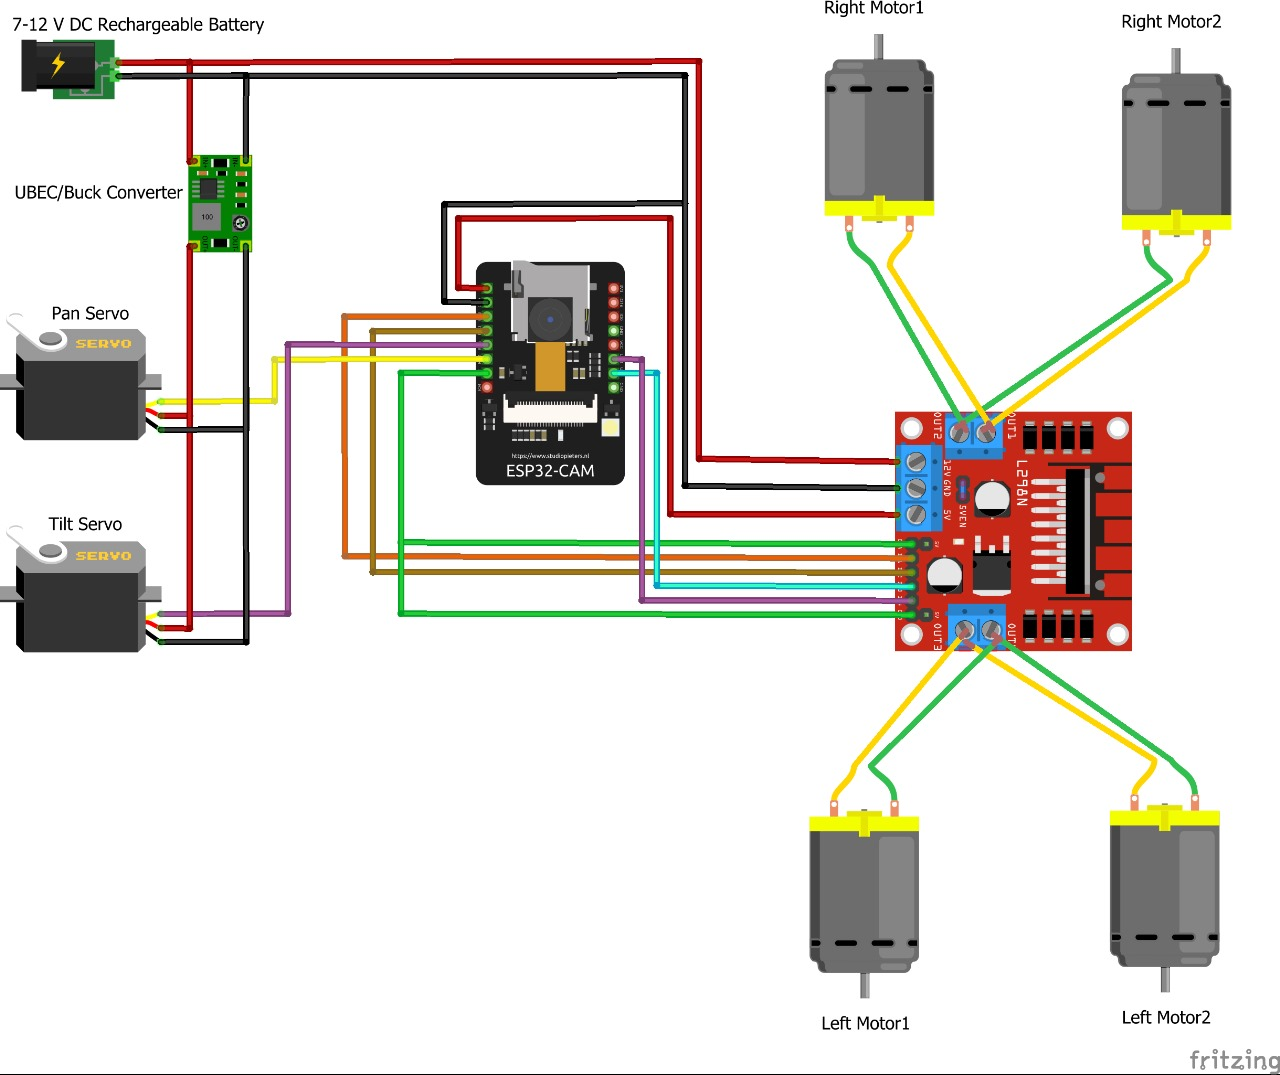
\includegraphics[width=1.0\linewidth]{bld.jpg}
    \caption{The diagram shows the connections between the 4WD motors with L298N motor driver, ESP-32 microcontroller, the Pan-tilt servo assembly and the batteries}
    \label{fig:enter-label}
\end{figure}

\newpage
\subsection{ESP-32 connection with Computer}\\
We will use the ESP-32's WiFi capabilities to host a web-server which the controlling device will connect with hotspot and enter the IP address of the ESP-32 module. The controlling device can control the Robot's wheels and the rotate servo motors by using the buttons in the website. The ESP-32 module will also send the video/photo stream to the computer, the website which is hosted by the ESP-32 will run ML models inside the controlling device for object detection. 
\begin{figure}[h]
    \centering
    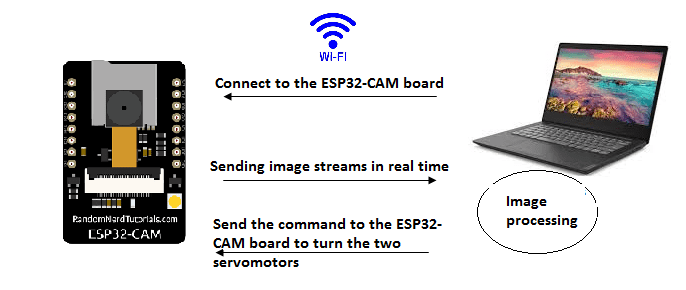
\includegraphics[width=0.75\linewidth]{com_esp.png}
    \caption{{the connections between the ESP-32 microcontroller and the computer or controlling device}}
    \label{fig:enter-label}
\end{figure}
\begin{figure}[h]
    \centering
    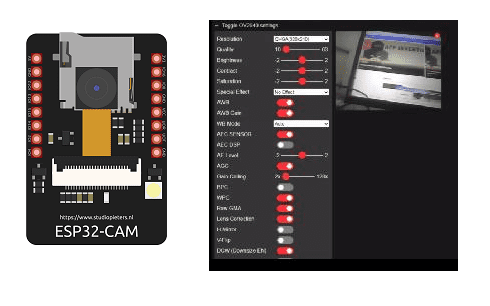
\includegraphics[width=0.75\linewidth]{esp32-cam-single.png}
    \caption{Demo Website Interface for controlling the robot}
    \label{fig:enter-label}
\end{figure}

\newpage

\section{Components Specification}
\newline
\begin{itemize}
    \item \textbf{ESP-32 Cam Module with Dev Board:}
    \begin{itemize}
        \item \textbf{Description:} A development board featuring the ESP-32 microcontroller with an integrated camera. It supports Wi-Fi and Bluetooth connectivity, making it ideal for wireless surveillance and IoT applications.
        \item \textbf{Role in Project:} Acts as the central processing unit and camera for capturing images and video, as well as handling wireless communication for remote control and streaming.
    \end{itemize}
    \begin{figure}[h]
        \centering
        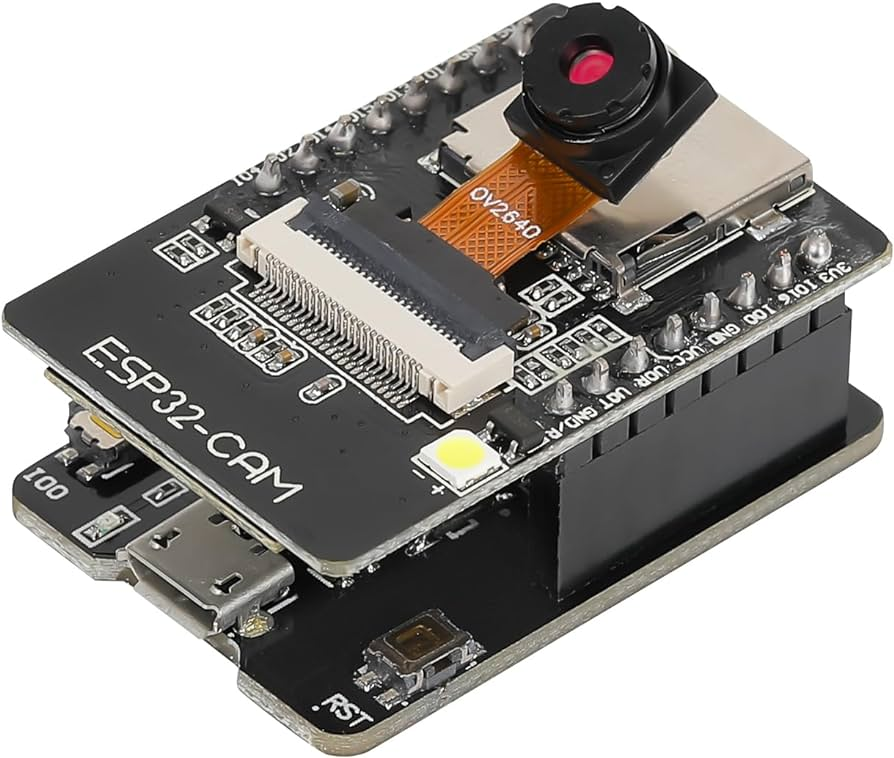
\includegraphics[width=0.25\linewidth]{image.png}
        \caption{ESP32 Cam module with Dev board}
        \label{fig:enter-label}
    \end{figure}

    \item \textbf{L298n Motor Driver Module:}
    \begin{itemize}
        \item \textbf{Description:} A dual H-bridge motor driver module that allows control of the speed and direction of two DC motors.
        \item \textbf{Role in Project:} Controls the DC motors in the 4WD car kit, enabling movement and navigation of the surveillance bot.
    \end{itemize}
    \begin{figure}[h]
        \centering
        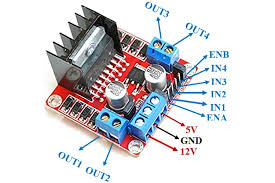
\includegraphics[width=0.4\linewidth]{images.jpeg}
        \caption{L298n Motor Driver}
        \label{fig:enter-label}
    \end{figure}
    \newpage
    \item \textbf{Pan Tilt Servo Assembly:}
    \begin{itemize}
        \item \textbf{Description:} A mechanical assembly that allows two-axis movement (pan and tilt) using two SG-90 servo motors.
        \item \textbf{Role in Project:} Provides the mechanism to adjust the camera angle, allowing the bot to capture images and videos from different perspectives.
    \end{itemize}
    \begin{figure}[htbp]
    \centering
    \begin{subfigure}[b]{0.45\textwidth}
        \centering
        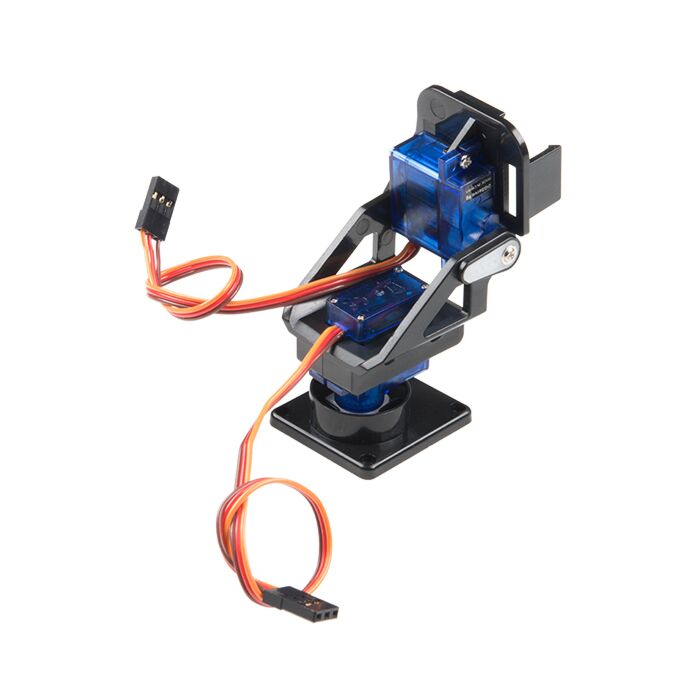
\includegraphics[width=0.5\linewidth]{pan_tilt.jpg}
        \caption{Pan-Tilt assembly}
        \label{fig:enter-label}
    \end{subfigure}
    \hfill
    \begin{subfigure}[b]{0.45\textwidth}
        \centering
        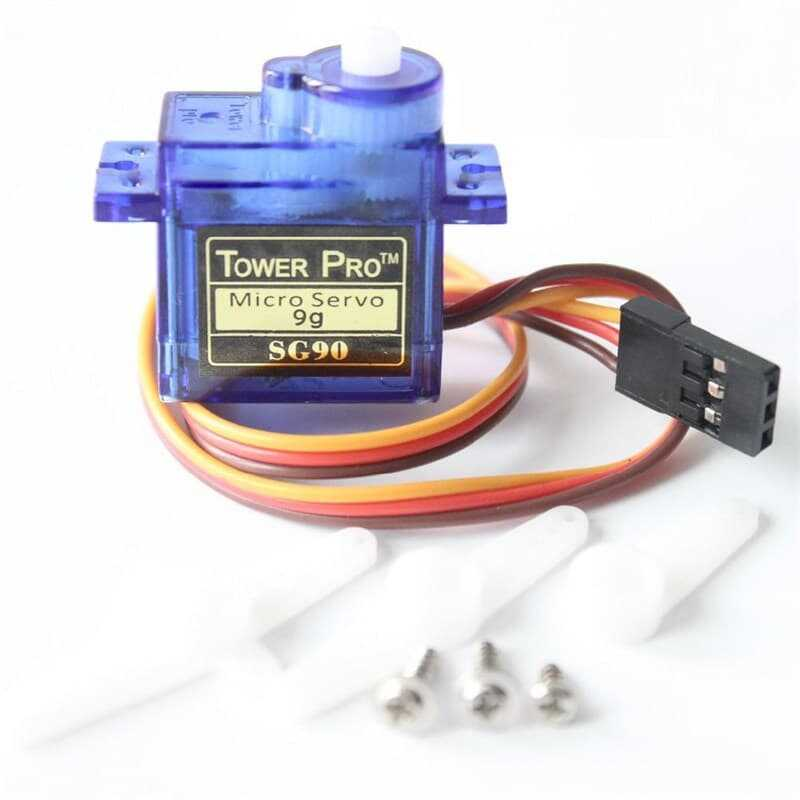
\includegraphics[width=0.5\linewidth]{sg90.jpg}
        \caption{SG90 Servos}
        \label{fig:enter-label}
    \end{subfigure}
    \caption{Pan-tilt Servo Assembly}
    \label{fig:side_by_side}
    \end{figure}

    \item \textbf{4WD Car Kit:}
    \begin{itemize}
        \item \textbf{Description:} A chassis kit with four-wheel drive, including a platform, wheels, and motors.
        \item \textbf{Role in Project:} Serves as the mobile base for the surveillance bot, providing mobility and the ability to navigate different terrains.
    \end{itemize}
    \begin{figure}[h]
        \centering
        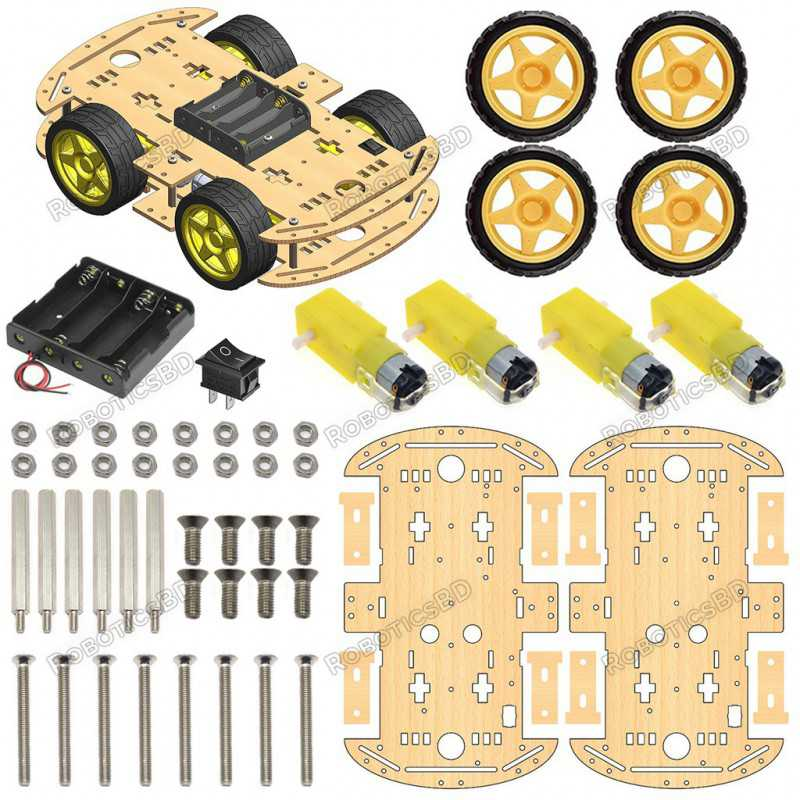
\includegraphics[width=0.4\linewidth]{4wd_.jpg}
        \caption{4WD Car with components}
        \label{fig:enter-label}
    \end{figure}
    \newpage
    \item \textbf{7-12V Rechargeable Battery:}
    \begin{itemize}
        \item \textbf{Description:} Rechargeable batteries that provide the necessary power for the bot and its components.
        \item \textbf{Role in Project:} Supplies power to the ESP-32 board, motors, and other electronics, ensuring the bot can operate without being tethered to a power source.
    \end{itemize}
    \begin{figure}[h]
        \centering
        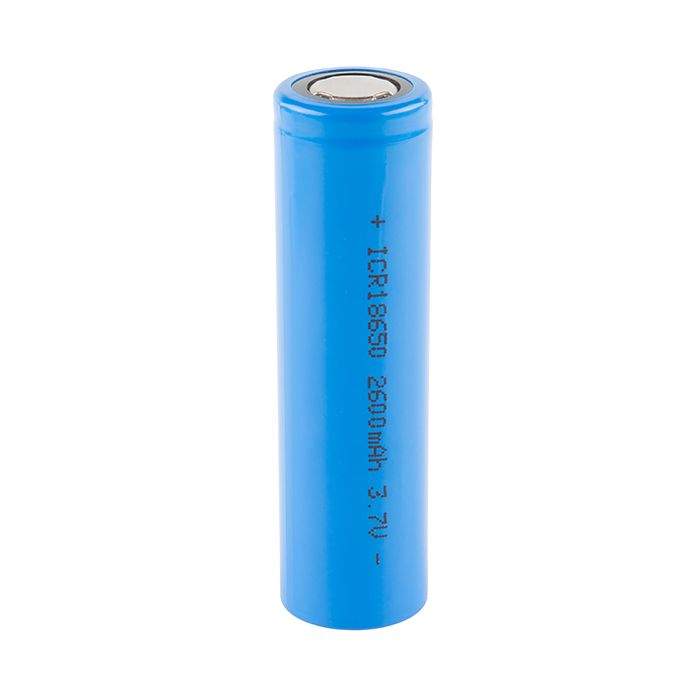
\includegraphics[width=0.15\linewidth]{batt.jpg}
        \caption{18650 Batteries}
        \label{fig:enter-label}
    \end{figure}

    \item \textbf{UBEC or Buck Converter:}
    \begin{itemize}
        \item \textbf{Description:} A voltage regulator that steps down the input voltage to a stable lower output voltage.
        \item \textbf{Role in Project:} Ensures that the voltage supplied to the ESP-32 and other components is within safe operating limits.
    \end{itemize}
    \begin{figure}[h]
        \centering
        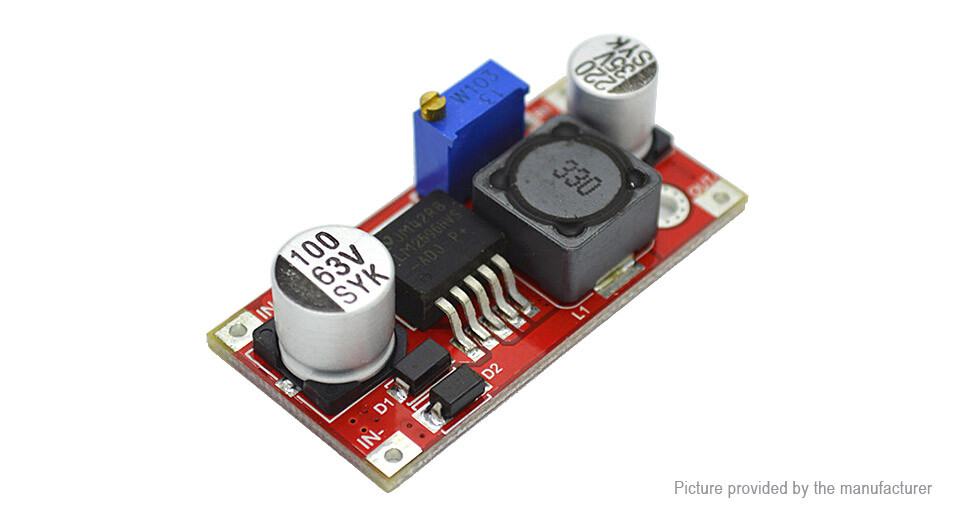
\includegraphics[width=0.25\linewidth]{buck converter.jpeg}
        \caption{Buck converter}
        \label{fig:enter-label}
    \end{figure}

    \item \textbf{Heatsink:}
    \begin{itemize}
        \item \textbf{Description:} A passive heat exchanger that absorbs and dissipates heat from electronic components.
        \item \textbf{Role in Project:} Attached to the ESP-32 or other heat-generating components to improve heat dissipation and maintain optimal operating temperature.
    \end{itemize}
    \begin{figure}[h]
        \centering
        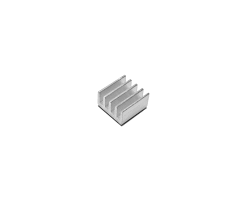
\includegraphics[width=0.15\linewidth]{sink.png}
        \caption{Heatsink}
        \label{fig:enter-label}
    \end{figure}
    
\end{itemize}

\newpage
\section{Components List}
\begin{table}[h!]
\centering
\Large
\begin{tabular}{|c|p{5cm}|c|c|}
\hline
\textbf{Serial} & \textbf{Name} & \textbf{Quantity} & \textbf{Cost (taka)} \\
\hline
1 & ESP-32 Cam module Dev board & 1 & 850 \\
\hline
2 & L298n motor driver module & 1 & 200 \\
\hline
3 & Pan Tilt Servo assembly & 1 & 130 \\
\hline
4 & Pan servo & 1 & 140 \\
\hline
5 & Tilt servo & 1 & 140 \\
\hline
6 & SG90 servo motors & 2 & 380 \\
\hline
7 & 4WD car kit & 1 & 900 \\
\hline
8 & 7-12V Rechargeable battery & 2 & 1300 \\
\hline
9 & UBEC or buck converter & 1 & 90 \\
\hline
10 & Jumper wires & 30 & 120 \\
\hline
11 & Heatsink & 1 & 50 \\
\hline
\multicolumn{3}{|r|}{\textbf{Total:}} & \textbf{4300 taka} \\
\hline
\end{tabular}
\caption{Table of components with cost analysis (approximation)}
\label{tab:cost_analysis}
\end{table}


% ----------------------------------------------------------------------
% Conclusion
% ----------------------------------------------------------------------
\section{Conclusion}
In conclusion, this remote controlled surveillance bot project provides a cost-effective and accessible solution for real-time monitoring and security applications. Its compact design, combined with wireless control and real-time streaming capabilities, makes it a versatile tool for various surveillance needs.


\end{document}
